% Template for Cogsci submission with R Markdown

% Stuff changed from original Markdown PLOS Template
\documentclass[10pt, letterpaper]{article}

\usepackage{cogsci}
\usepackage{pslatex}
\usepackage{float}
\usepackage{caption}

% amsmath package, useful for mathematical formulas
\usepackage{amsmath}

% amssymb package, useful for mathematical symbols
\usepackage{amssymb}

% hyperref package, useful for hyperlinks
\usepackage{hyperref}

% graphicx package, useful for including eps and pdf graphics
% include graphics with the command \includegraphics
\usepackage{graphicx}

% Sweave(-like)
\usepackage{fancyvrb}
\DefineVerbatimEnvironment{Sinput}{Verbatim}{fontshape=sl}
\DefineVerbatimEnvironment{Soutput}{Verbatim}{}
\DefineVerbatimEnvironment{Scode}{Verbatim}{fontshape=sl}
\newenvironment{Schunk}{}{}
\DefineVerbatimEnvironment{Code}{Verbatim}{}
\DefineVerbatimEnvironment{CodeInput}{Verbatim}{fontshape=sl}
\DefineVerbatimEnvironment{CodeOutput}{Verbatim}{}
\newenvironment{CodeChunk}{}{}

% cite package, to clean up citations in the main text. Do not remove.
\usepackage{apacite}

% KM added 1/4/18 to allow control of blind submission


\usepackage{color}

% Use doublespacing - comment out for single spacing
%\usepackage{setspace}
%\doublespacing


% % Text layout
% \topmargin 0.0cm
% \oddsidemargin 0.5cm
% \evensidemargin 0.5cm
% \textwidth 16cm
% \textheight 21cm

\title{Response Times as Negative Evidence in Grammar Learning}


\author{{\large \bf Morton Ann Gernsbacher (MAG@Macc.Wisc.Edu)} \\ Department of Psychology, 1202 W. Johnson Street \\ Madison, WI 53706 USA \AND {\large \bf Sharon J.~Derry (SDJ@Macc.Wisc.Edu)} \\ Department of Educational Psychology, 1025 W. Johnson Street \\ Madison, WI 53706 USA}


\begin{document}

\maketitle

\begin{abstract}
Include no author information in the initial submission, to facilitate
blind review. The abstract should be one paragraph, indented 1/8 inch on
both sides, in 9\textasciitilde point font with single spacing. The
heading `Abstract' should be 10\textasciitilde point, bold, centered,
with one line of space below it. This one-paragraph abstract section is
required only for standard six page proceedings papers. Following the
abstract should be a blank line, followed by the header `Keywords' and a
list of descriptive keywords separated by semicolons, all in
9\textasciitilde point font, as shown below.

\textbf{Keywords:}
Add your choice of indexing terms or keywords; kindly use a semi-colon;
between each term.
\end{abstract}

Children rapidly learn to use language to successfully communicate with
others, despite receiving little formal instruction about how to use
language before attending school. How do children learn so much about
language so quickly? Children are great at pulling linguistic
information from others' speech and using those patterns to make
predictions. Saffran, Aslin, and Newport (1996) showed that
prelinguistic infants can follow statistical regularities in speech
streams to detect word boundaries, and they can generate these patterns
to novel sequences (Aslin \& Newport, 2012). Therefore, children receive
a large amount of positive evidence -- information about what is correct
to say -- from their social partners. However, within the English
language, there are a lot of exceptions to patterns and rules. Is
listening to examples from adults enough information for children to
master language?

Children are not only passive listeners of language, but they also
become active participants in conversations. Through interacting with
caregivers, they might learn from the corrections adults give to their
mistakes. For example, if a child pointed to a horse and said ``dog!'',
a parent might respond ``that's not a dog, that's a horse!'' However,
adults are much less likely to correct syntactic errors (Newport,
Gleitman, \& Gleitman, 1977). For example, if a child said ``I falled''
instead of ``I fell'', a parent is much less likely to directly point
out the error, because the content of their speech was correct.
Nonetheless, children are able to learn and use accurate grammar. If
children are not regularly told which utterances are ungrammatical, how
do they quickly become proficient communicators?

One possibility is that parents give children implicit corrections when
they speak ungrammatically. For example, parents are more likely to
reformulate their child's utterance, in other words repeating it with
corrected grammar, when their child makes an error (Hirsh-Pasek,
Treiman, \& Schneiderman, 1984, p. @chouinard2003). So, when their child
says ``I falled'', parents might respond ``you fell!'' The child may be
able to use the contrast between their own utterance and their parent's
response as negative evidence -- evidence their utterance was
ungrammatical-- and learn from their parent's example. Children are
better at learning novel grammatical rules when they receive these
reformulations than when they're only given correct examples unrelated
to their speech (Saxton et al., 1998). Therefore, children do seem able
to detect and use this implicit cue for learning in a controlled
context.

However, parents do not consistently reformulate their children's
errors. While parents are more likely to repeat an utterance when they
are correcting their child, they do still often repeat correct
utterances (Chouinard \& Clark, 2003). Therefore, children may struggle
to detect that the parent intended to correct rather than simply respond
with a repetition (Marcus, 1993, p. @morgan1989). If children use
repetition rates as evidence alone, Marcus (1993) argues that a child
would need to make the same mistake over 80 times for them to notice a
difference in how the parent responds. On the other hand, Saxton (2000)
argues that the linguistic contrast between the parent and child's
utterances is salient enough, without requiring the child to track
repetition rates to use this cue. How do children learn from this
unreliable signal?

We hypothesize that another, more implicit cue, might indicate to the
child that the parent noticed an error. Adults are slower to process
unpredictable utterances, therefore, timing may serve as a low-level cue
that the child has made an error (Jurafsky, 1999; Fine \& Jaeger, 2013).
The longer pause combined with the linguistic contrast between the
parent's and child's utterances may then serve as sufficient negative
evidence against their mistakes. We investigate whether parents take
longer to respond to their child's ungrammatical utterances, and explore
processing demands as a possible explanation for why parents might be
slower to respond.

\hypertarget{corpus-study-1}{%
\section{Corpus Study 1}\label{corpus-study-1}}

In this first study, we aimed to explore whether parents' response times
after ungrammatical and grammatical utterances differ consistently
during real interactions. Since the errors children make are highly
variable, we specified our analysis to a specific and clear grammatical
error: overregularizations. Overregularizations are instances where a
child incorrectly generalizes a grammatical rule, such as adding -s to
the end of a noun to designate plurality, or adding -ed to the end of a
verb to refer to past tense. For example, saying ``mouses'' instead of
``mice'' or ``runned'' instead of ``ran'' would be an
overregularization. To detect whether there is difference in how long
parents take to respond to their child's errors, we compared parent
response times after overregularizations and grammatical utterances
where the child produced a correct plural or past tense.

\hypertarget{methods}{%
\subsection{Methods}\label{methods}}

\hypertarget{child-data.}{%
\subsubsection{Child data.}\label{child-data.}}

Analyses were performed using the Eleanor, Fraser, and Thomas corpora
from the CHILDES database (MacWinney, 2000). Children are likely to
produce overregularizations from age 2 up until ages 5 or 6 (Marcus et
al., 1992). Therefore, these corpora were chosen because of their age
range, high recording frequency, and the availability of timing data.
Child utterances were selected that were responded to by the parent, and
contained valid time codes for both the child utterance and parent
response. These utterances also had to contain a past-tense or a plural.
Data were extracted from the XML versions of the database using a Python
script to parse the transcriptions. For both the Thomas and Fraser
corpora, the father's responses were removed because the number of
responses were negligible compared to that of the mother (0.23\% and
5.75\% of utterances, respectively). For the Eleanor corpus, both
parents were included because they both contributed significantly, and
their response patterns did not vary significantly.

\hypertarget{coding.}{%
\subsubsection{Coding.}\label{coding.}}

We hand-coded whether utterances tagged with an error were an
overregularization or an ``other error.'' `` Other error'' refers to
utterances in which the child made an error was not due to an
overregularization of the past tense or plural. For example, the
utterance ``it did go elephants sleep'' contains a plural
(``elephants'') and past tense, but the error is not an error of
overregularization. Cases where the time of the utterance was longer
than 5 seconds, less than 5 seconds, or utterance longer than 9 seconds
were marked as suspicious timing. We verified whether these utterances
were indeed marked with correct timings and whether the response was a
contextual response to the child's utterance. If the utterance passed
this criterion, it was included in the analysis.

\begin{CodeChunk}
\begin{figure*}[h]

{\centering 
\includegraphics{figs/2-col-image-1} 

}

\caption[This image spans both columns]{This image spans both columns. And the caption text is limited to 0.8 of the width of the document.}\label{fig:2-col-image}
\end{figure*}
\end{CodeChunk}

\hypertarget{one-column-images}{%
\subsection{One-column images}\label{one-column-images}}

Single column is the default option, but if you want set it explicitly,
set \texttt{fig.env} to \texttt{figure}. Notice that the
\texttt{num.cols} option for the caption width is set to \texttt{1}.

\begin{CodeChunk}
\begin{figure}[H]

{\centering 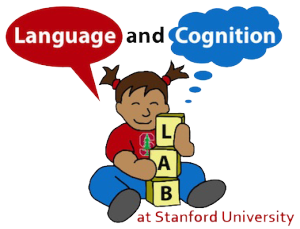
\includegraphics{figs/image-1} 

}

\caption[One column image]{One column image.}\label{fig:image}
\end{figure}
\end{CodeChunk}

\hypertarget{r-plots}{%
\subsection{R Plots}\label{r-plots}}

You can use R chunks directly to plot graphs. And you can use latex
floats in the fig.pos chunk option to have more control over the
location of your plot on the page. For more information on latex
placement specifiers see
\textbf{\href{https://en.wikibooks.org/wiki/LaTeX/Floats,_Figures_and_Captions}{here}}

\begin{CodeChunk}
\begin{figure}[H]

{\centering 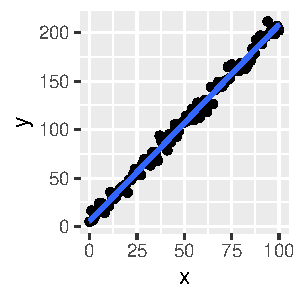
\includegraphics{figs/plot-1} 

}

\caption[R plot]{R plot}\label{fig:plot}
\end{figure}
\end{CodeChunk}

\hypertarget{tables}{%
\subsection{Tables}\label{tables}}

Number tables consecutively; place the table number and title (in 10
point) above the table with one line space above the caption and one
line space below it, as in Table 1. You may float tables to the top or
bottom of a column, set wide tables across both columns.

You can use the xtable function in the xtable package.

\begin{table}[H]
\centering
\begin{tabular}{rrrrr}
  \hline
 & Estimate & Std. Error & t value & Pr($>$$|$t$|$) \\ 
  \hline
(Intercept) & 0.02 & 0.11 & 0.2 & 0.84 \\ 
  x & 1.79 & 0.13 & 14.0 & 0.00 \\ 
   \hline
\end{tabular}
\caption{This table prints across one column.} 
\end{table}

\hypertarget{acknowledgements}{%
\section{Acknowledgements}\label{acknowledgements}}

Place acknowledgments (including funding information) in a section at
the end of the paper.

\hypertarget{references}{%
\section{References}\label{references}}

\setlength{\parindent}{-0.1in} 
\setlength{\leftskip}{0.125in}

\noindent

\hypertarget{refs}{}
\leavevmode\hypertarget{ref-chouinard2003}{}%
Chouinard, M. M., \& Clark, E. V. (2003). Adult reformulations of child
errors as negative evidence. \emph{Journal of Child Language},
\emph{30}(3), 637--670.

\leavevmode\hypertarget{ref-hirsh-pasek1984}{}%
Hirsh-Pasek, K., Treiman, R., \& Schneiderman, M. (1984). Brown \&
hanlon revisited: Mothers' sensitivity to ungrammatical forms.
\emph{Journal of Child Language}, \emph{11}(1), 81--88.

\leavevmode\hypertarget{ref-marcus1993}{}%
Marcus, G. F. (1993). Negative evidence in language acquisition.
\emph{Cognition}, \emph{46}(1), 53--85.

\leavevmode\hypertarget{ref-morgan1989}{}%
Morgan, J. L., \& Travis, L. L. (1989). Limits on negative information
in language input. \emph{Journal of Child Language}, \emph{16}(3),
531--552.

\leavevmode\hypertarget{ref-newport1977}{}%
Newport, E., Gleitman, H., \& Gleitman, L. R. (1977). Mother i'd rather
do it myself: The contribution of selected child listener variables'.

\bibliographystyle{apacite}


\end{document}
